
\chapter{Related Concepts}\label{chp:related}
First, we are going to explore related concepts and research relevant to our topic. This chapter provides an overview on related language modelling techniques, interpretability of language models and grammatical inference.

\section{Language Modelling}
Language modelling is generally used to provide algorithms with an understanding of natural language and generate human-like texts.

\dfn{Language Model}{
    Let $\Sigma$ denote an alphabet of tokens. A language model $M$ assigns a string of tokens $w_1, \ldots, w_n \in \Sigma^n$ an estimated probability $P(w_1, \ldots, w_n)$ or $P(w_i \mid w_1, \ldots, w_{i-1})$ for all $1 \leq i \leq n$, based on distributions seen in a training corpus $T \in \Sigma^N$ of length $N$.\par
}
\noindent
The language model considers a string of tokens $w = w_1, \ldots, w_n$ as a time-discrete stochastic process $X_1, \ldots, X_n$, where each token position is a random variable over an alphabet or vocabulary $\Sigma$. The model estimates the probability of a given string $w$ by predicting the assignments to these random variables. We write $P(X_1 = w_1, X_2 = w_2, \ldots, X_n = w_n)$ or $P(w_1, \ldots, w_n)$ for the probability of the tokens $w_1, \ldots, w_n$.
From the chain rule of probabilities we know that~\cite{parsing2009speech}:
\begin{align*}
    P(w_1, \ldots, w_n) = P(w_1)*P(w_2 \mid w_1)*\ldots*P(w_n \mid w_1, \ldots, w_{n-1})
\end{align*}

\noindent
This means that a language model both models the conditional probabilities $P(w_i \mid w_1, \ldots, w_{i-1})$ for all $1 \leq i \leq n$ and the probabilities of given sequences. Another way to see this relationship is the definition of conditional probability:
\begin{align*}
    P(A \mid B) = \frac{P(A \cap B)}{P(B)}
\end{align*}
Which can be applied to sequences of tokens in the following way:
\begin{align*}
    P(w \mid w_1, \ldots, w_{i-1}) = \frac{P(w_1, \ldots, w_i)}{P(w_1, \ldots, w_{i-1})}
\end{align*}

\noindent
A basic model to estimate these probability distributions is the \textit{n-Gram model}.
\dfn{N-Gram Model}{
    An n-gram of order $n$ is a string $w^n$ of $n$ tokens. An \textit{n-gram model} stores counts of all n-grams appearing in a given corpus $T \in \Sigma^*$. A count function $C(\cdot): \Sigma^n \rightarrow \NN$ maps each n-gram to the number of times it occurs in $T$. The probability of a token $w_i$ following $n-1$ given tokens can then be calculated using the counts for n-grams of order $n$ and $n-1$:
    \begin{align*}
        P(w_i \mid w_{i-n+1}, \ldots, w_{i-1}) = \frac{C(w_{i-n+1}, \ldots, w_i)}{C(w_{i-n+1}, \ldots, w_{i-1})}
    \end{align*}
}\label{def:n-gram}
\noindent
Intuitively, an n-gram model counts the portion of occurrences of the $(n-1)$-gram in the corpus which have been followed by the token $w_i$. This way it estimates the token at position $i$ from the given context of $n-1$ tokens.

N-grams are however limited by their order $n$ in how much preceding context it can include during prediction. Relationships beyond this context window are not captured by a single n-gram model, which is one of its major drawbacks, as natural language contains long-range dependencies.

Increasing the value of $n$ can quickly increase the number of counts having to be stored, as the number of n-grams to be counted can grow exponentially. The number of possible n-grams over an alphabet $\Sigma$ of size $|\Sigma| = k$ is given by $k^n$. Although a corpus $T$ of length $N$ can only contain at most $N - n + 1$ $n$-grams for a given length $n$, large corpora are long enough for the number of possible n-grams to be counted to become unpractical.

\noindent
To precisely model the probability of a token given an arbitrary context, n-gram models would need to store n-grams of arbitrary length. As this would often require a lot of space to store the various possible n-grams, usually the n-gram length is limited. It is possible to estimate the true probability of each n-gram given in the corpus by only looking at a limited context size. This assumes the Markov property on the stochastic process and helps limit the memory required for the n-grams:
\dfn{Markov Property}{
    A stochastic process $X_1, \ldots, X_N$ is said to possess the Markov property of order $n$ if:
    \begin{align*}
        P(X_i \mid X_{1}, \ldots, X_{i-1}) = P(X_i \mid X_{i - n}, \ldots, X_{i-1})
    \end{align*}
    That is the probability of the $i$-th state only depends on the past $n$ states. A stochastic process with this property is also called an $n$-th order Markov Chain.
}
\noindent
A Markov chain of order $1$ is also called \textit{memoryless}, as its next state only depends on the current state. N-gram models make the assumption that the stochastic process of the language they are modelling possesses the Markov property and that the probability of a token conditioned on the entire context can be approximated with a limited context window:
\begin{align*}
    P(w_i \mid w_{1}, \ldots, w_{i-1}) \approx P(w_i \mid w_{i - n + 1}, \ldots, w_{i-1})
\end{align*}

\section{Distributional Semantics}

In the research field of distributional semantics, the similarity between linguistic 
items is defined as the similarity of their respective context distributions in a 
given text corpus. The distributional hypothesis proposes that ``words which 
appear in similar contexts are similar in their meaning'' or ``words are 
characterized by the company they keep''.

\noindent
Various methods for capturing context information for language modelling have been developed, most notably Word2Vec~\cite{mikolov2013efficient} has been used to learn \emph{word embeddings} from the contexts the words occur in. Word embeddings being high-dimensional real-valued vectors, optimized using gradient-descent, which can easily be used for similarity comparison and arithmetic calculations in a hyper-dimensional semantic space. They represent words based on their distributional semantic meaning and allow for relatively robust predictions of surrounding contexts, however as iteratively optimized hyper-dimensional vectors they are usually difficult to interpret while also being lossy representations of the context.

\section{Attention Mechanism}
N-gram models have since been superseded by recurrent neural networks (RNNs), LSTM (Long-Short Term Memory) networks and then Transformers~\cite{VaswaniSPUJGKP17}, a self-attention based neural architecture. Transformers are designed to \textit{transform} a sequence of input tokens into another by incorporating context information from the input tokens into each output token. Transformers use word embeddings to represent individual tokens and during training, they learn \textit{attention weights} between all directed pairs of tokens in the vocabulary. The attention weights allow the model to more efficiently incorporate context information into its latent representations by learning the relative importance of words in the context.

\dfn{Scaled Dot-Product Self-Attention}{
    Let $X \in \RR^{n \times d}$ be the matrix of $d$-dimensional word embedding for the $n$ input tokens. Further, let $\mathbf{W_K} \in \RR^{d \times d_k}$, $\mathbf{W_Q} \in \RR^{d \times d_k}$ and $\mathbf{W_V} \in \RR^{d \times d_v}$ be the \textit{key}, \textit{query} and \textit{value} weight matrices, mapping each word embedding $x_i$ to its respective key, query and value vectors $k_i$, $q_i$ and $v_i$.
    \begin{align*}
        \mathbf{K} = \mathbf{XW_K},\quad
        \mathbf{Q} = \mathbf{XW_Q},\quad
        \mathbf{V} = \mathbf{XW_V}
    \end{align*}
    Such that $\mathbf{K} \in \RR^{n \times d_k}$, $\mathbf{Q} \in \RR^{n \times d_k}$ and $\mathbf{V} \in \RR^{n \times d_v}$ contain $k_i$, $q_i$ and $v_i$ for all $n$ input tokens in their rows.
    The self-attention mechanism computes the output embedding for each input token $i$ as a weighted sum of all the value vectors $j$ in $\mathbf{V}$, where the weight is the dot product of the associated $q_i$ and $k_j$ vectors, scaled by the inverse root of the key and query vector dimension:
    \begin{align*}
        \text{Attention}(\mathbf{Q}, \mathbf{K}, \mathbf{V}) = \text{softmax}\left(\frac{\mathbf{Q}\mathbf{K}^T}{\sqrt{d_k}}\right)\mathbf{V}
    \end{align*}
}
The associated $q_i$ and $k_i$ vectors can be viewed as positions of the ``sending'' and ``receiving'' endpoints in a ``\textit{link space}'', where the similarity of two vectors corresponds to the attention weight the first token assigns to the other. With this representation, tokens with similar contexts in the training data are assigned similar endpoints in the link space during training. This allows the transformer model to easily generalize from the training data and predict similar context even if they never occurred in the training data, simply based on the similarity of each token's latent representation.

%\noindent
%The transformer architecture as it was presented in \citetitle{VaswaniSPUJGKP17} trains more than one set of attention weight matrices which it calls \textit{multi-head attention}. Each set of $\mathbf{(W_Q, W_K, W_V)}$ is called an \textit{attention head}. This way the model can learn different assignments of attention weights between tokens, which allows it to learn different types of relationships between tokens and helps learn dependencies over longer distances.
%
%\section{Attention Visualisation}
%
%\begin{figure}[ht!]
%    \centering
%    %\hspace{-1cm}
%    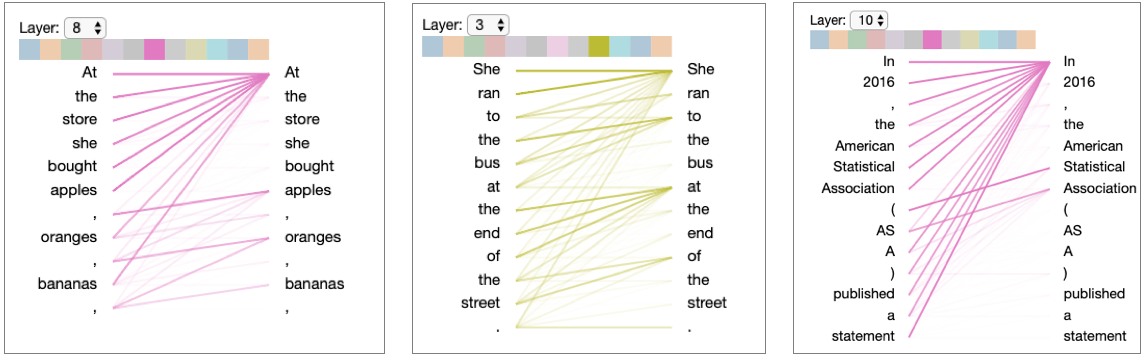
\includegraphics[scale=0.4]{images/attention2}
%    \caption{Attention-Head visualisations generatated by the BertViz tool.}
%\end{figure}
%
%The issue of interpretability in neural networks, or the lack thereof, has often been recognized and discussed. Many approaches to visualizing the weights of neural networks have been made, with varying success.  
%

\section{Grammar Induction}

As opposed to neural networks, formal grammars are a rule-based approach to model a language. A formal grammar is generally defined as a set of \emph{production rules} producing valid examples of a target language.
\dfn{Formal Grammar}{
    A formal grammar $G = (V, \Sigma, P, S)$ is represented by
    \begin{itemize}[itemsep=0em]
        \item $V$, a finite vocabulary of symbols used in the production rules
        \item $\Sigma$, a set of terminal symbols, called the alphabet
        \begin{itemize}[itemsep=0em]
            \item $N = V \setminus \Sigma$, is the set of non-terminal symbols
        \end{itemize}
        \item $P \subset (V^* \setminus \Sigma^*) \times V^*$, a finite set of production rules, mapping strings of symbols with at least one non-terminal to other strings of symbols
        \item $S \in N$, a starting symbol
    \end{itemize}
}
\noindent
Using a formal grammar, a language $L(G)$, which is defined as a set of strings, can be recognized and generated by a finite automaton. The task of learning such a grammar from a given set of examples of a language is called \emph{grammar induction}. There are many approaches to this task from trial and error, over evolutionary algorithms to greedy inference of appropriate rules to represent the given examples.

Loss-less compression algorithms such as the Lempel-Ziv-Welch algorithm also qualify as grammatical induction, as they construct a grammar to represent the input with fewer symbols by deduplication. The Sequitur~\cite{nevill1997identifying} algorithm has been used to reveal hierarchical structure in sequences such as text and music, by detecting repetitions in the data. Further, many modern neural architectures use grammar induction algorithms such as byte pair encoding~\cite{zouhar2023formal} in their tokenization step to compress the training data while maintaining some awareness for the substructure of words. This shows that grammar induction is not only a means to reduce memory consumption, but also to identify significant structure of the input which can help modelling of the data.

Although much research in the field of grammar induction exists, we have not found a grammatical induction algorithm that is able to relate all frequent substrings of an input with their respective contexts in the input. As this is crucial information used by state-of-the-art language models such as the transformer, and since the context is a defining part of to the general concept of distributional semantics, we set out to build an algorithm to induce such a grammar.

